
\section{Buckley Leverett Equations with/without Gravity} 

\subsection{Nomenclature}
\begin{tabular}{c l}
%\hline
%
$f_{j}$: & fractional flow of phase $j$ \\
%
$f_{ij}$: & $\partial f_{i}/\partial S_{j}$ \\
%
$g$: & gravitational acceleration constant \\
%
$j$: & phase \\
%
$k$: & absolute permeability of the porous medium in 1D \\
%
$k_{rj}$:& relative permeability of phase $j$ \\
%
$k^{o}_{rj}$: & endpoint relative permeability of phase $j$ \\
%
$n_{j}$: & Corey exponent of phase $j$\\
%
$n_{p}$: & number of phases present\\
%
$S_{j}$: & saturation of phase $j$\\
%
$S_{j}^{\star}$: & normalized saturation of phase $j$\\
%
$S_{rj}$: & residual saturation of phase $j$\\
%
$v$: & flow velocity in 1D\\
%
$\mu_{j}$: & viscosity of phase $j$\\
%
$\rho_{mj}$: & mass density of phase $j$\\
%
$\lambda$: & eigenvalue (characteristic velocity)\\
%
$\Lambda$: & shock velocity\\
%
$\theta$: & dip angle of porous medium from horizontal\\
%
%\hline
\end{tabular}



\subsection{Equations}

Using the notation and derivation of \cite{Orr_2007}, the conservation equations for purely convective one-dimensional flow of two immiscible phases is

\begin{eqnarray}
&&\frac{{\partial S_j }}{{\partial \tau }} +  \frac{{\partial f_j }}{{\partial \xi }}  = 0 \label{eqn:BL}\\
&&j = g,w,o \nonumber
\end{eqnarray}

\noindent where dimensionless time $\tau = \frac{v t}{\phi L}$ and dimensionless distance $\xi = \frac{x}{L}$ .  For the two-phase water/gas system only one of these equations is independent as $S_g + S_w = 1$.  All variables are defined in the Nomenclature section.

The fractional flow of a component is defined as

\begin{eqnarray}
&&f_j = \frac{\frac{k_{rj}}{\mu_j}}{\sum_{n=1}^{n_p}{\frac{k_{rn}}{\mu_n}}} \left( 1-\frac{kg \sin \theta}{v} \sum_{n=1}^{n_p}{\frac{k_{rn}}{\mu_n}\left( \rho_{mj}-\rho_{mn} \right)} \right) \label{eqn:ff}
\end{eqnarray}

\noindent where

\begin{eqnarray}
&&k_{rj} = k_{rj}^o {\left(S_j^*\right)^{n_j}}\\
&&S_j^* = \frac{S_j - S_{rj}}{1-\sum_{n=1}^{n_p}{S_{rn}}} \nonumber
\end{eqnarray}

\noindent which can be written entirely in terms of $S_g$ for the Buckley-Leverett problem using $S_w = 1-S_g$.  Equation \ref{eqn:BL} can be solved as an eigenvalue problem by ...

The exact analytical form for the derivative of the fractional flow is

\begin{eqnarray}
\frac{df_g}{dS_g}&=& \frac{\left(\frac{\frac{d k_{rg}}{d S_g}}{\mu_g}\right) \frac{k_{rw}}{\mu_w}-\left(\frac{\frac{d k_{rw}}{d S_g}}{\mu_w}\right)\frac{k_{rg}}{\mu_g}}{\left(\frac{k_{rg}}{\mu_g}+\frac{k_{rw}}{\mu_w}\right)^2}\left( 1-\frac{kg \sin \theta}{v} \frac{k_{rw}}{\mu_w}\left( \rho_{mg}-\rho_{mw} \right) \right)\nonumber \\
&&-f_g\frac{kg \sin \theta}{v} \frac{\frac{d k_{rw}}{d S_g}}{\mu_w}\left(\rho_{mg}-\rho_{mw} \right)
\end{eqnarray}

\noindent where

\begin{eqnarray}
\frac{d k_{rg}}{d S_g} &=& k_{rg}^o n_g \frac{\left(S_g - S_{rg}\right)^{n_g-1}}{\left(1-S_{rg}-S_{rw}\right)^{n_g}}\nonumber \\
\frac{d k_{rw}}{d S_g}&=& -k_{rw}^o n_w \frac{\left(1-S_g - S_{rw}\right)^{n_w-1}}{\left(1-S_{rg}-S_{rw}\right)^{n_w}}\nonumber 
\end{eqnarray}



\subsection{Parameters in example problems}
All parameters in Equation \ref{eqn:BL} are assumed to be constant in the Buckley-Leverett problem.  The fractional flow parameters are given in Table \ref{table:paras}.

\begin{table}[h]
\begin{center}
\begin{tabular}{lrrrr}
\hline
Phase&$S_{rj}$&$k_{rj}^o$&$n_j$& $\mu_j$($cp$)\\
%%\lcline{1-1}\rlcline{2-5}
Gaseous&0.1&1.0&2.0&0.1\\
%Oleic&-&-&-&-\\
Aqueous&0.3&1.0&2.0&1.0\\
\hline
\end{tabular}
\caption{Fractional flow parameters for the benchmark Cases I-III.}
\label{table:paras}
\end{center}
\end{table}


\subsection{Solutions}

\subsubsection{Case I: Solution without gravity}
The first benchmark solution is for the case of no gravity, i.e. a horizontal displacement.  The initial (right state) and injection (left state) conditions are given in Table \ref{table:BCs}.

\begin{table}[h]
\begin{center}
\begin{tabular}{lrr}
\hline
BC & $S_g$ & $S_w$\\
%%\lcline{1-1}\rlcline{2-3}
Initial& 0.0 & 1.0\\
(right state)&  & \\
Injection&1.0 & 0.0\\
(left state)&  & \\
\hline
\end{tabular}
\caption{Boundary conditions for benchmark Cases I-III. }
\label{table:BCs}
\end{center}
\end{table}



\begin{figure}[h]
\centering
%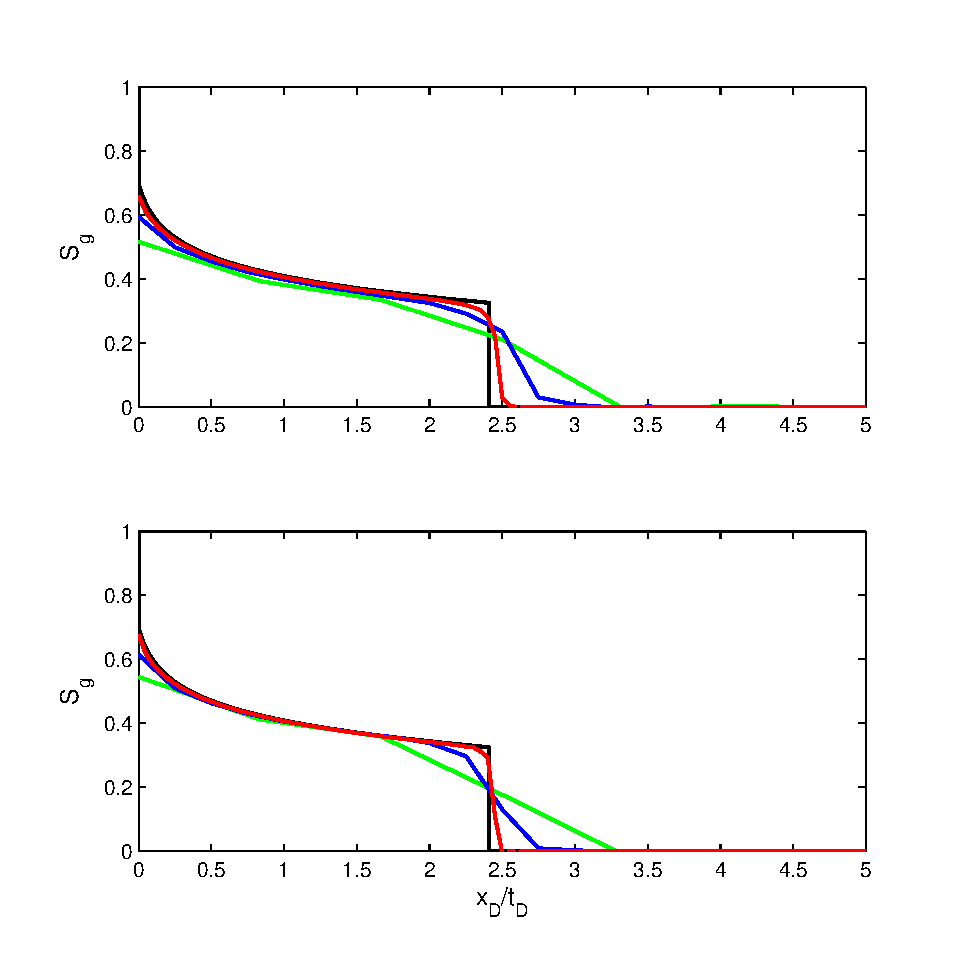
\includegraphics[width=0.75\textwidth,viewport=10 10 420 420,clip]{./figures/BL_no_gravity}
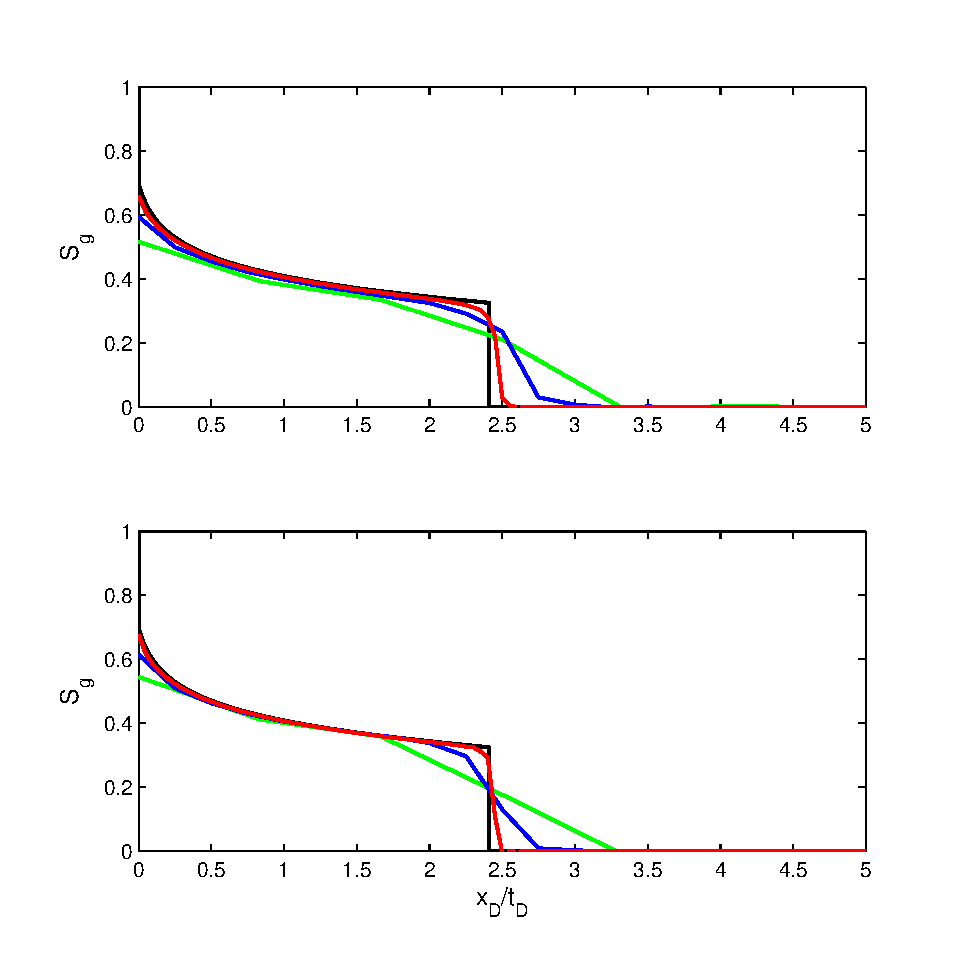
\includegraphics[width=10.0cm,height=15.cm]{./figures/BL_no_gravity}
\vspace{-4.cm}
\caption{Top: Comparison the analytical solutions to Case I without gravity with the upstream weighted DG simulated solution with for 3 (green), 10 (blue) and 50 (red) grid blocks.  Bottom: Comparison the analytical solutions to Case I without gravity with the mixed weighted DG simulated solution for 3 (green), 10 (blue) and 50 (red) grid blocks.} 
\label{fig:BL_no_grav}
\end{figure}


The displacement consists of a fast moving shock wave from the initial condition, with no gas, to a gas saturation of $S_g = 0.3255$, followed by a rarefaction wave to the residual water saturation. As there is no transfer of components between phases, it is impossible to move the residual water from the system.

The DG simulator was run in 2 modes, upstream weighting and 80\% upstream weighting.  A comparison of the analytical solution for various levels of refinement is shown for upstream weighting on the top of Figure \ref{fig:BL_no_grav} and for mixed weighting on the bottom. 

\paragraph{Displacements with gravity}

In this case the flux in the conservation law is slightly different.  The fractional flow curve as computed from Eq. \ref{eqn:ff} may be larger than one or less than zero, which is physically meaningless in one dimension as $f_g$ is defined as the fraction of the total flow that is taken up by the gas phase.  The impossible fluxes are caused by the inability of a 1D model to capture counter-current gravity-driven flow.  A 2D benchmark case to study this effect will be dealt with later.  Anytime Eq. \ref{eqn:ff} gives $f_g > 1.0$ it must be that in 1D $f_g = 1.0$, similarly if $f_g < 0.0$ in Eq. \ref{eqn:ff}, $f_g = 0.0$.  The additional parameters necessary for the cases including gravity are in Table \ref{table:grav_const}.  The phase densities are calculated using the method from \cite{spycher_2003}.


\begin{table}[h]
\begin{center}
\begin{tabular}{lr}
\hline
$\rho_g$ ($\frac{kg}{m^3}$)& 710 \\
%$\rho_o$ ($\frac{kg}{m^3}$)&-\\
$\rho_w$ ($\frac{kg}{m^3}$)& 1050\\
g ($\frac{m^2}{s}$)& 9.8 \\
k ($ m^2$)& $9.87E-13$\\
v ($ \frac{m}{s}$)& $5.00E-06$\\
\hline
Case II &\\
$\theta$ (degrees) & -90 \\
\hline
Case III &\\
$\theta$  (degrees)& 90  \\
\hline
\end{tabular}
\caption{Additional parameters needed for benchmark Cases II and III with gravity. Phase densities for water and super-critical CO$_2$ are at 80$^oC$ and 27$MPa$. }
\label{table:grav_const}
\end{center}
\end{table}



\paragraph{Case II: Displacements with gravity slowing displacement}

The first benchmark solution including gravity is the injection of oil into the bottom of a vertical core or sand pack. In this case analytical solution in the presence of gravity is physically meaningful, though there is a small region at low $S_g$ where $f_g < 0.0$.  The solution structure is the same as in the displacement without gravity.  Because the more dense oil is being pushed into the core against the force of gravity the leading shock front and rarefaction wave have both slowed down substantially.


\begin{figure}[h]
\vspace{-1cm}
\centering
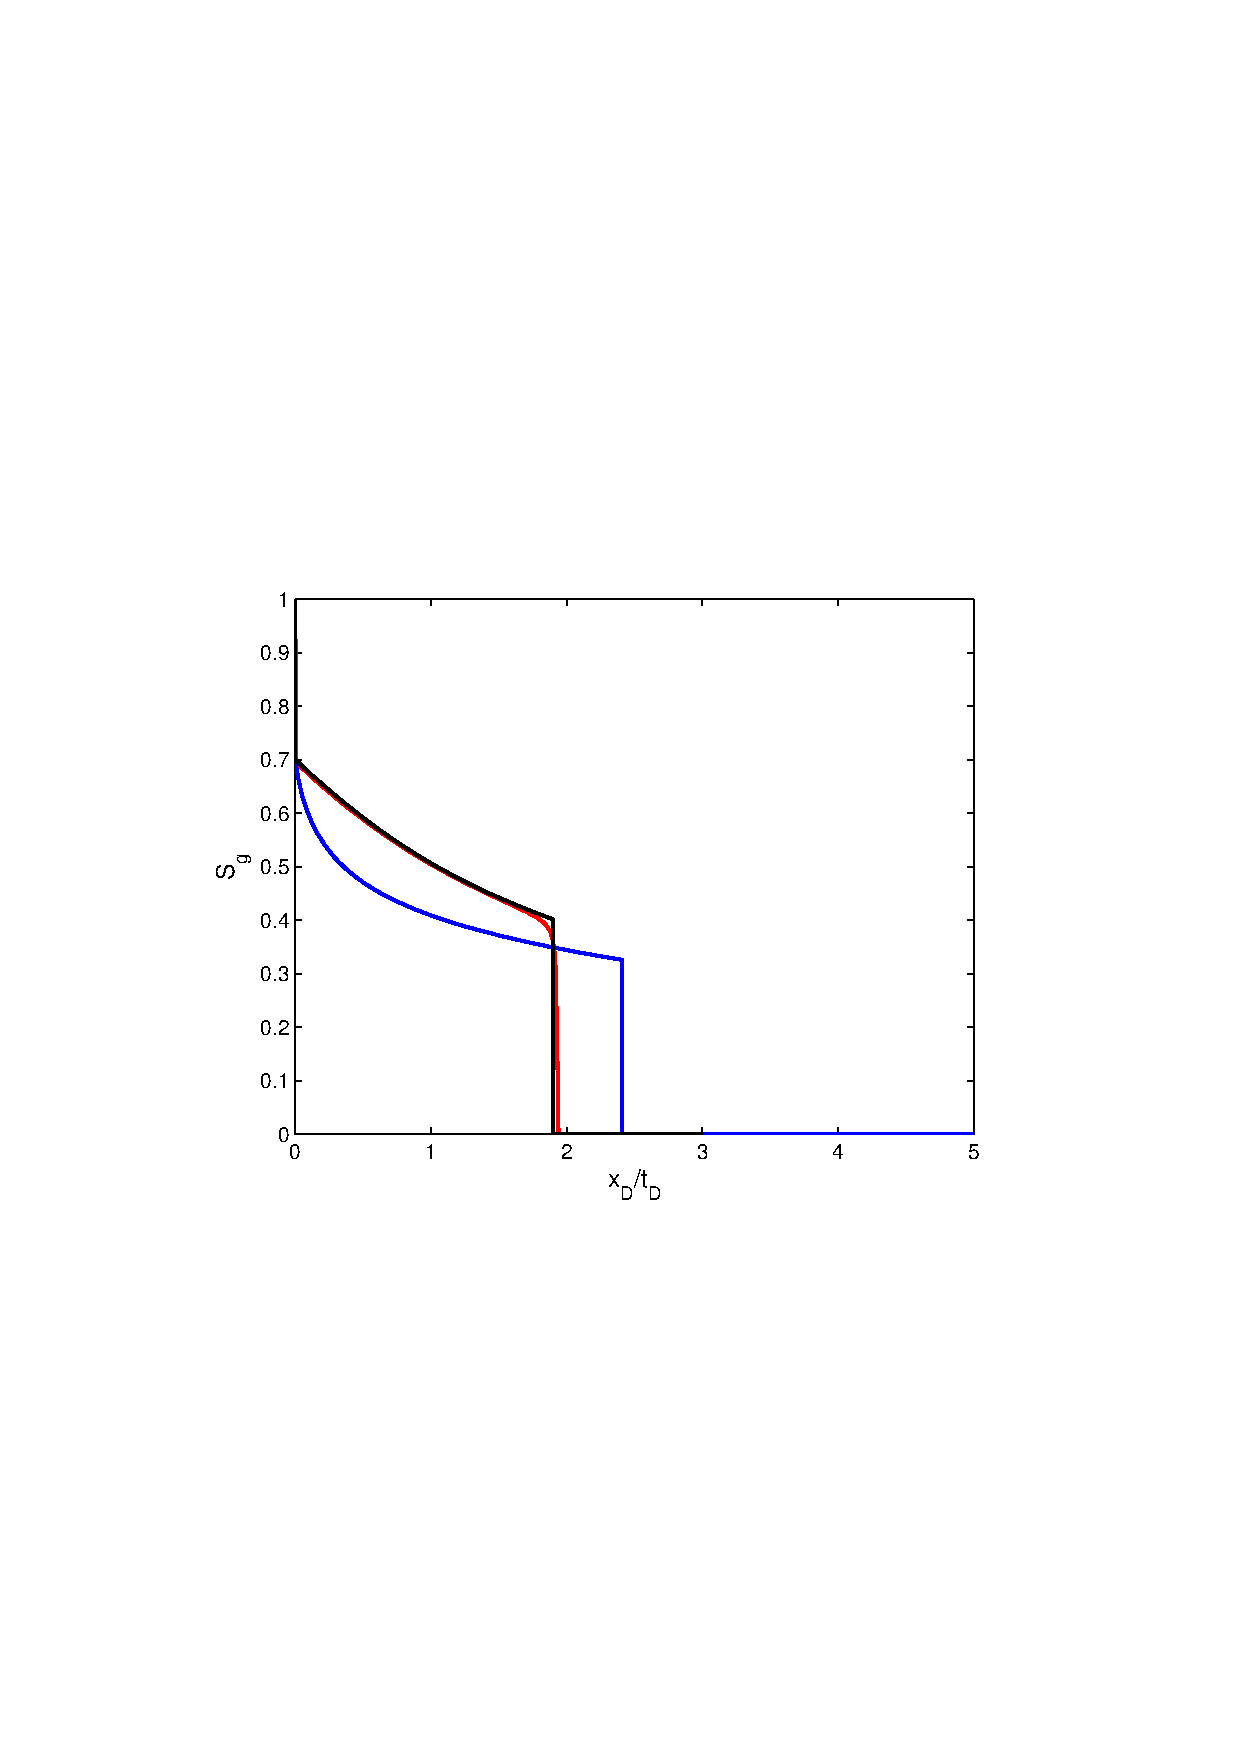
\includegraphics[width=15.0cm,height=20.cm]{./figures/BL_gravity_up}
%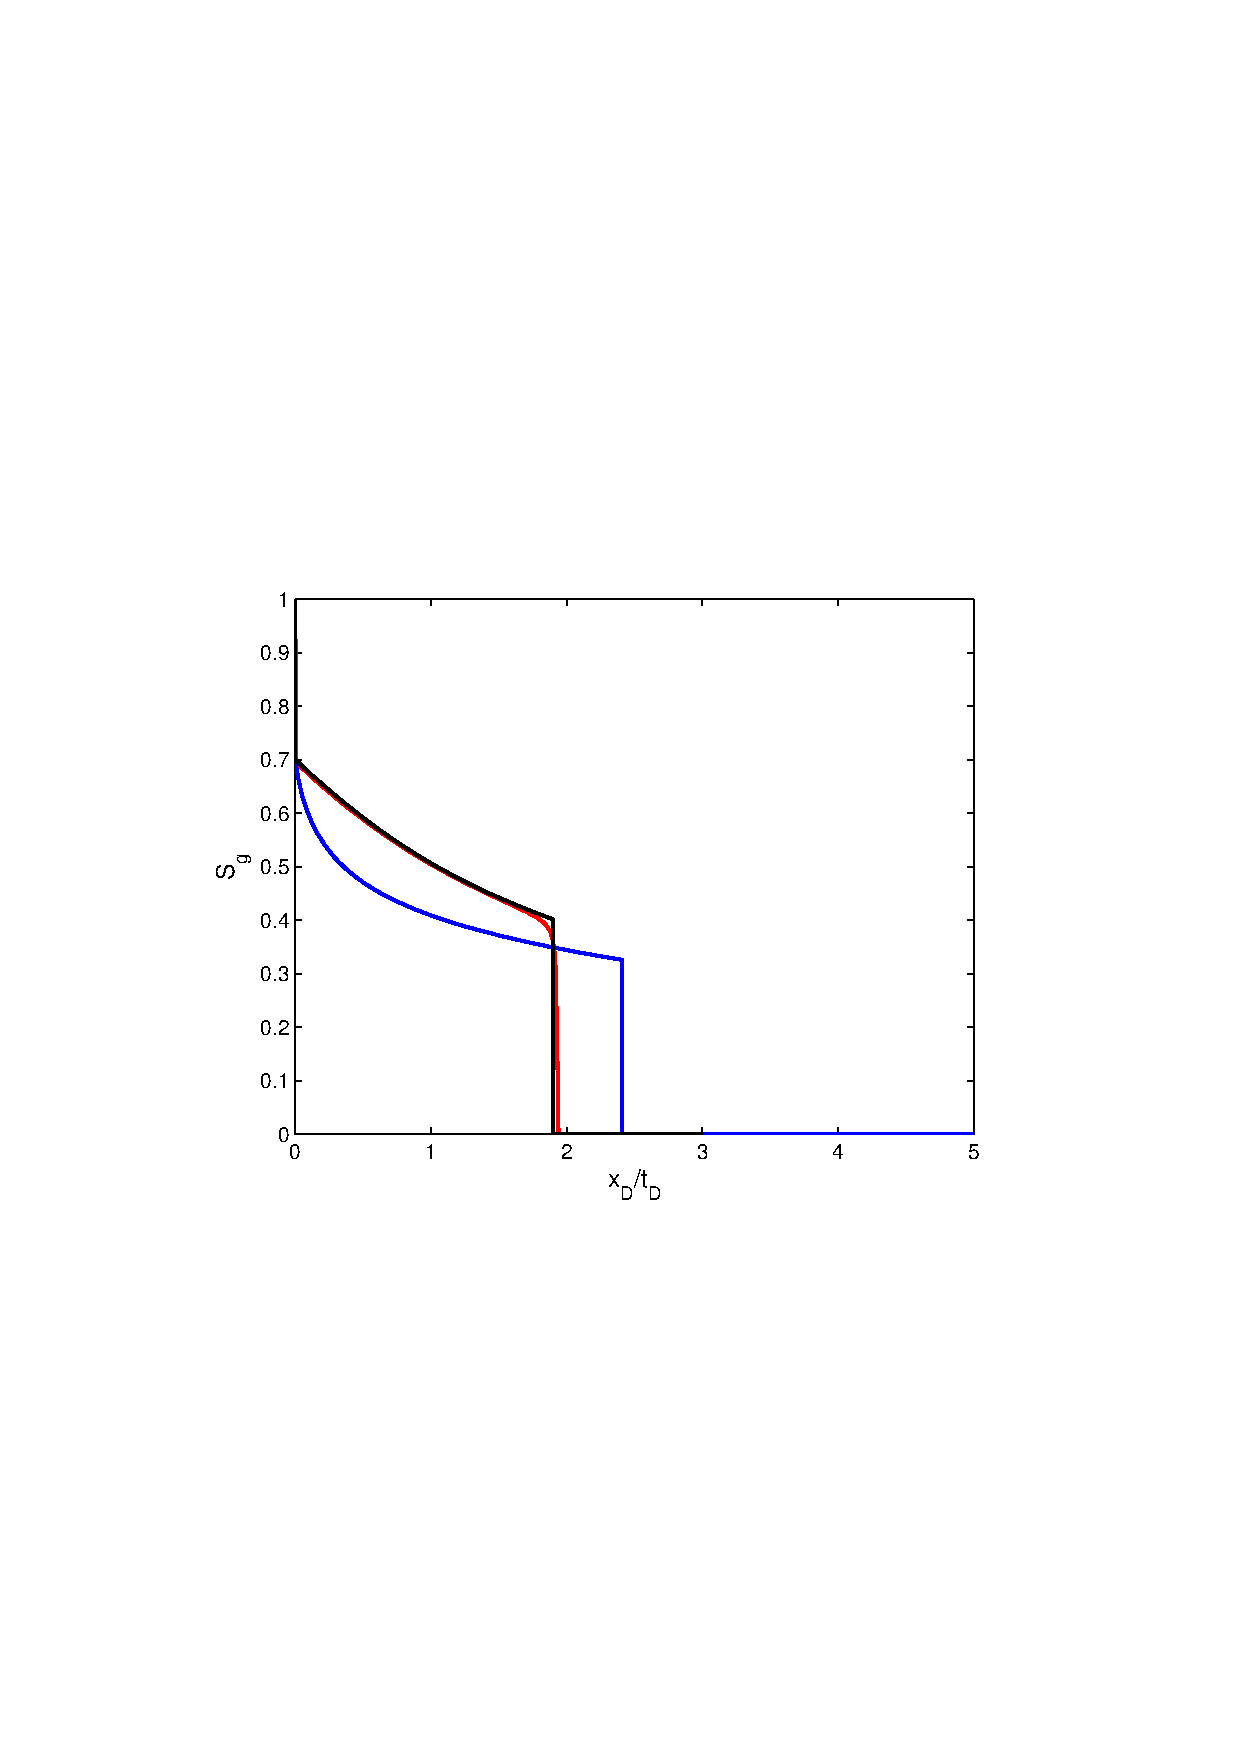
\includegraphics[width=0.75\textwidth,viewport=10 0 390 300,clip]{./figures/BL_gravity_up}
\vspace{-5.5cm}
\caption{Analytical solution to Case II, the stable benchmark case with gravity (black) slowing the displacement.  A fine-grid FD solution (red) and the analytical solution for the case without gravity (blue) are shown for comparison purposes.} 
\label{fig:BL_grav_up}
\end{figure}

\paragraph{Case III: Displacements with gravity accelerating displacement}

The second benchmark solution including gravity is the injection of oil into the top of a vertical core or sand pack. In reality this displacement is gravity unstable and needs to be modelled in two-dimensions, but for the purposes of benchmarking the code it is still useful. 

The solution with gravity is a shock wave from the right state to the saturation $S_g = 0.2960$ followed by a rarefaction wave to $S_g = 0.3340$.  Then there is a constant state to the injection composition.  This constant state is caused by the fact that $f_g > 1.0$ for large gas saturations and no longer tapers off uniformly as the residual water saturation is approached.

The analytical solution with gravity is shown in Figure \ref{fig:BL_grav_down} with a fine-grid FD solution and the analytical solution without gravity for comparison.  

\begin{figure}[h]
\vspace{-1cm}
\centering
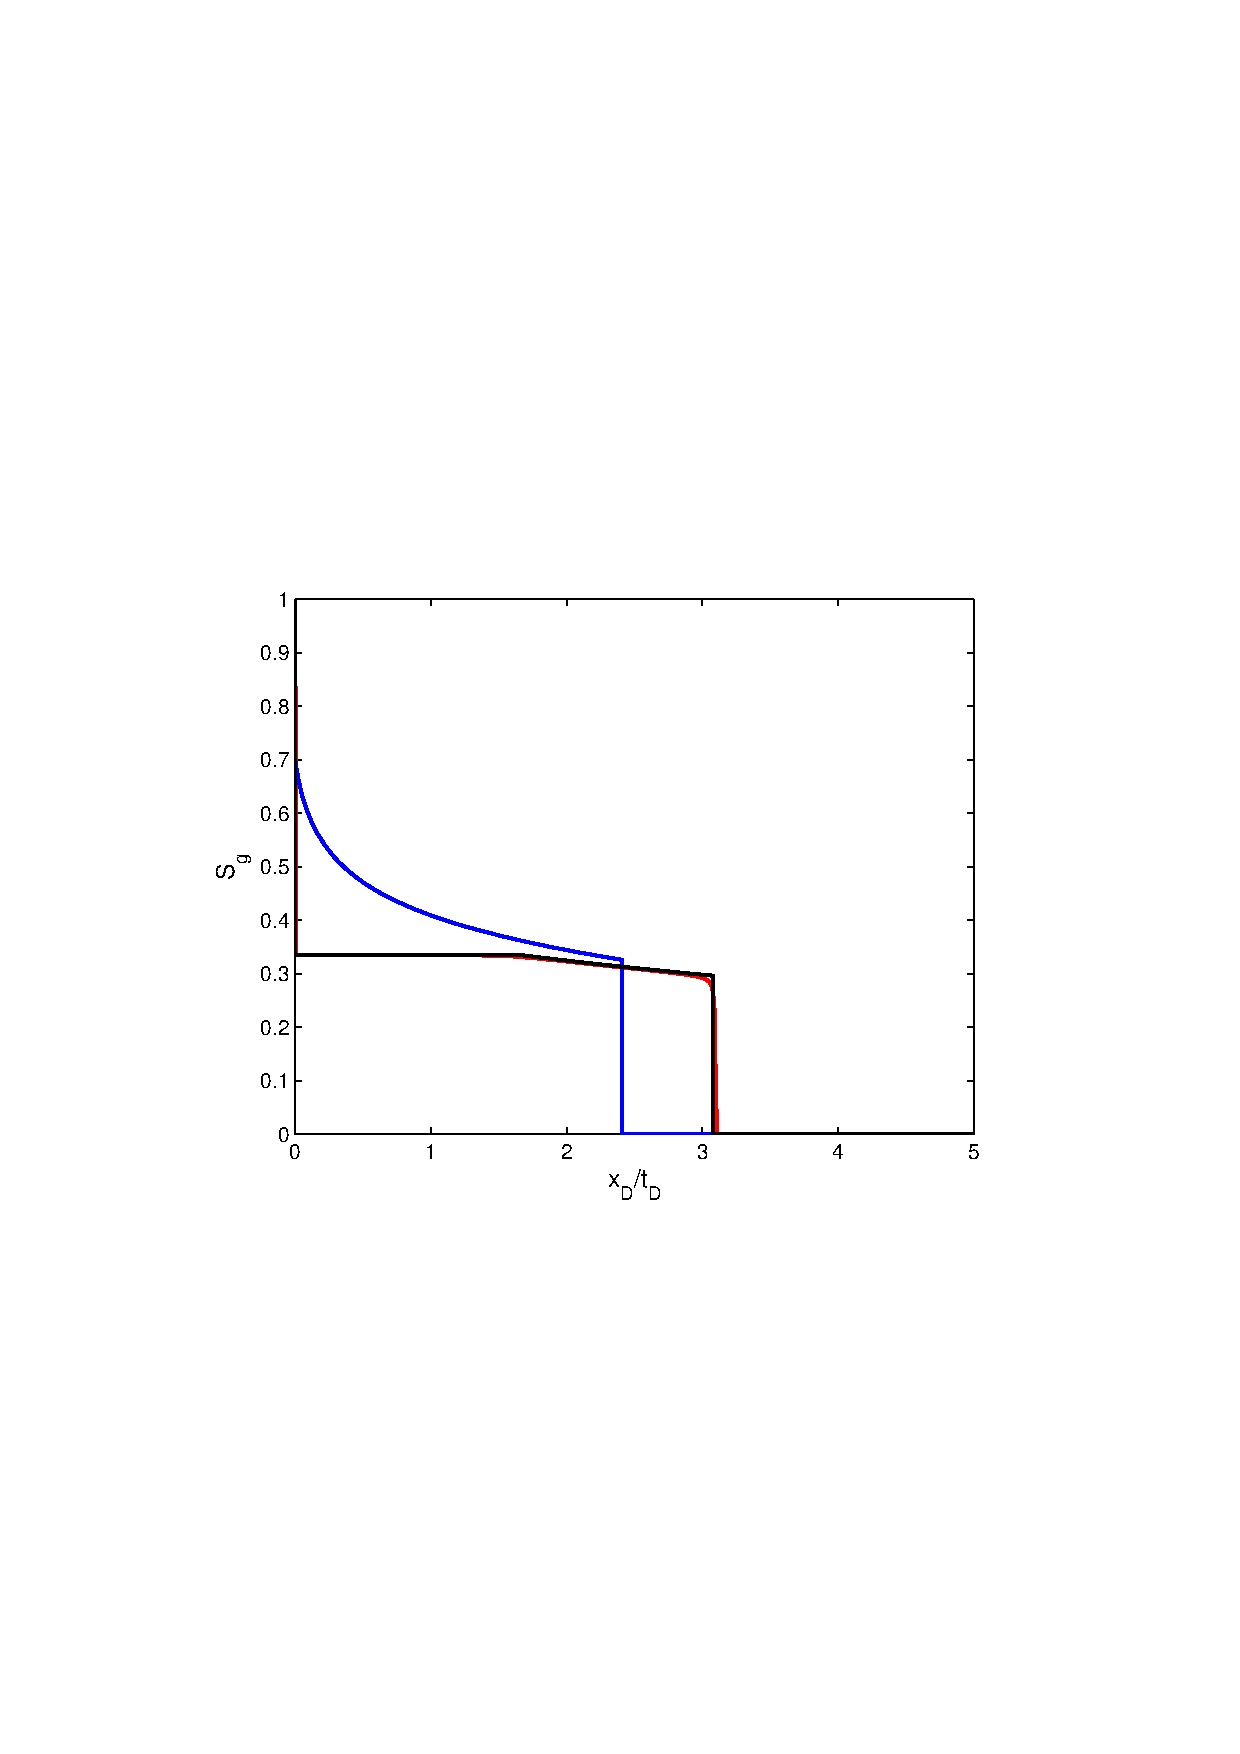
\includegraphics[width=15.0cm,height=20.cm]{./figures/BL_gravity_down}
\vspace{-5.5cm}
%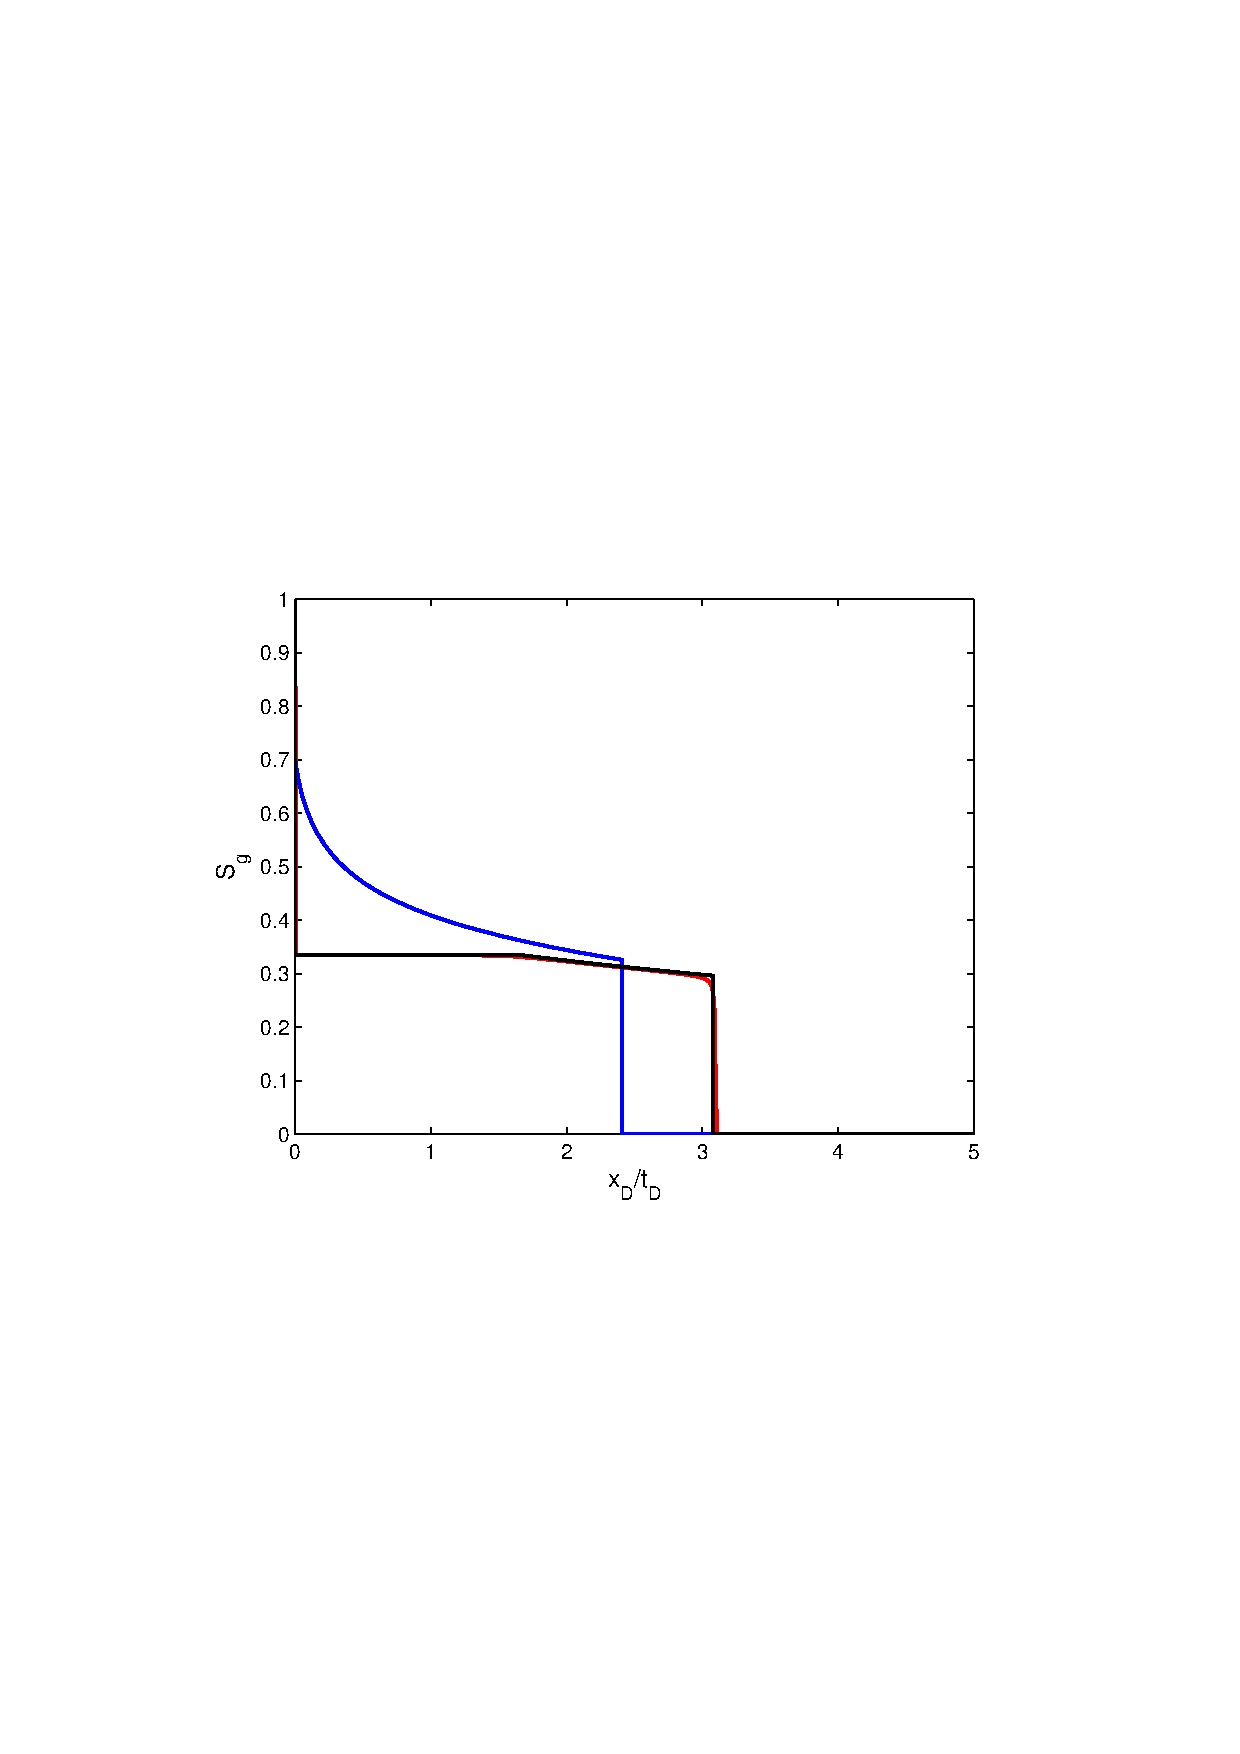
\includegraphics[width=0.75\textwidth,viewport=10 0 390 300,clip]{./figures/BL_gravity_down}
\caption{Analytical solution to Case III, the unstable benchmark case with gravity (black) accelerating the displacement.  A fine-grid FD solution (red) and the analytical solution for the case without gravity (blue) are shown for comparison purposes.} 
\label{fig:BL_grav_down}
\end{figure}

